%! TEX root = ../root/raiz.tex
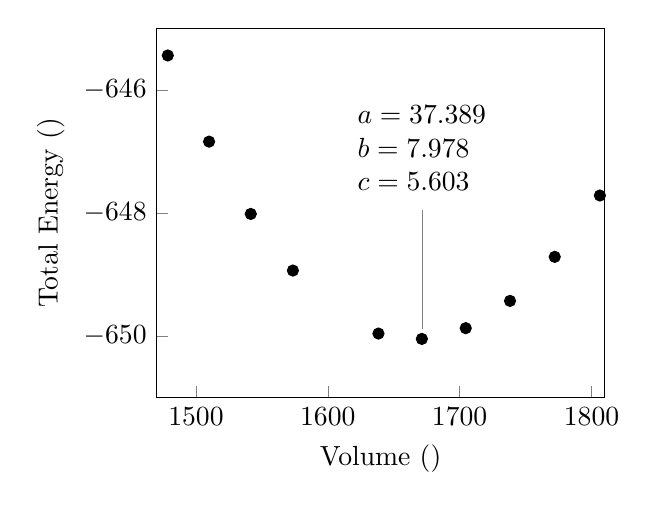
\begin{tikzpicture}
    \begin{axis}
        [
            width=.6\linewidth,
            legend pos={outer north east},
            legend style={draw=none},
            legend cell align=left,
            tick align=inside,
            tick pos=left,
            minor tick num=0,
            xlabel={Volume (\si{\cubic\angstrom})},
            xmin=1470,xmax=1810,
            xticklabel style={
                /pgf/number format/.cd,
                1000 sep={}
            },
            ylabel={Total Energy (\si{\electronvolt})},
            ymin=-651,ymax=-645
        ]
        \addplot [black, only marks, mark=*] table {
        1478.66 -645.44242760
        1509.96 -646.84113965
        1541.58 -648.01530539
        1573.53 -648.93434002
        1638.41 -649.95751005
        1671.34 -650.04437184
        1704.60 -649.86959858
        1738.19 -649.42708077
        1772.10 -648.71194118
        1806.35 -647.71591055
        }
        node [pin={[pin distance=10ex]90:\begin{tabular}{l}$a=\SI{37.389}{\angstrom}$\\$b=\SI{7.978}{\angstrom}$\\$c=\SI{5.603}{\angstrom}$\\\end{tabular}}] at (1671.34, -650.04437184) {};
    \end{axis}
\end{tikzpicture}
